% Options for packages loaded elsewhere
\PassOptionsToPackage{unicode}{hyperref}
\PassOptionsToPackage{hyphens}{url}
%
\documentclass[
  english,
  man,floatsintext]{apa6}
\usepackage{amsmath,amssymb}
\usepackage{lmodern}
\usepackage{ifxetex,ifluatex}
\ifnum 0\ifxetex 1\fi\ifluatex 1\fi=0 % if pdftex
  \usepackage[T1]{fontenc}
  \usepackage[utf8]{inputenc}
  \usepackage{textcomp} % provide euro and other symbols
\else % if luatex or xetex
  \usepackage{unicode-math}
  \defaultfontfeatures{Scale=MatchLowercase}
  \defaultfontfeatures[\rmfamily]{Ligatures=TeX,Scale=1}
\fi
% Use upquote if available, for straight quotes in verbatim environments
\IfFileExists{upquote.sty}{\usepackage{upquote}}{}
\IfFileExists{microtype.sty}{% use microtype if available
  \usepackage[]{microtype}
  \UseMicrotypeSet[protrusion]{basicmath} % disable protrusion for tt fonts
}{}
\makeatletter
\@ifundefined{KOMAClassName}{% if non-KOMA class
  \IfFileExists{parskip.sty}{%
    \usepackage{parskip}
  }{% else
    \setlength{\parindent}{0pt}
    \setlength{\parskip}{6pt plus 2pt minus 1pt}}
}{% if KOMA class
  \KOMAoptions{parskip=half}}
\makeatother
\usepackage{xcolor}
\IfFileExists{xurl.sty}{\usepackage{xurl}}{} % add URL line breaks if available
\IfFileExists{bookmark.sty}{\usepackage{bookmark}}{\usepackage{hyperref}}
\hypersetup{
  pdftitle={Item Characteristic Curves derived from CTT Item Statistics},
  pdfauthor={Diego Figueiras1 \& John T. Kulas1},
  pdflang={en-EN},
  pdfkeywords={keywords},
  hidelinks,
  pdfcreator={LaTeX via pandoc}}
\urlstyle{same} % disable monospaced font for URLs
\usepackage{graphicx}
\makeatletter
\def\maxwidth{\ifdim\Gin@nat@width>\linewidth\linewidth\else\Gin@nat@width\fi}
\def\maxheight{\ifdim\Gin@nat@height>\textheight\textheight\else\Gin@nat@height\fi}
\makeatother
% Scale images if necessary, so that they will not overflow the page
% margins by default, and it is still possible to overwrite the defaults
% using explicit options in \includegraphics[width, height, ...]{}
\setkeys{Gin}{width=\maxwidth,height=\maxheight,keepaspectratio}
% Set default figure placement to htbp
\makeatletter
\def\fps@figure{htbp}
\makeatother
\setlength{\emergencystretch}{3em} % prevent overfull lines
\providecommand{\tightlist}{%
  \setlength{\itemsep}{0pt}\setlength{\parskip}{0pt}}
\setcounter{secnumdepth}{-\maxdimen} % remove section numbering
% Make \paragraph and \subparagraph free-standing
\ifx\paragraph\undefined\else
  \let\oldparagraph\paragraph
  \renewcommand{\paragraph}[1]{\oldparagraph{#1}\mbox{}}
\fi
\ifx\subparagraph\undefined\else
  \let\oldsubparagraph\subparagraph
  \renewcommand{\subparagraph}[1]{\oldsubparagraph{#1}\mbox{}}
\fi
% Manuscript styling
\usepackage{upgreek}
\captionsetup{font=singlespacing,justification=justified}

% Table formatting
\usepackage{longtable}
\usepackage{lscape}
% \usepackage[counterclockwise]{rotating}   % Landscape page setup for large tables
\usepackage{multirow}		% Table styling
\usepackage{tabularx}		% Control Column width
\usepackage[flushleft]{threeparttable}	% Allows for three part tables with a specified notes section
\usepackage{threeparttablex}            % Lets threeparttable work with longtable

% Create new environments so endfloat can handle them
% \newenvironment{ltable}
%   {\begin{landscape}\centering\begin{threeparttable}}
%   {\end{threeparttable}\end{landscape}}
\newenvironment{lltable}{\begin{landscape}\centering\begin{ThreePartTable}}{\end{ThreePartTable}\end{landscape}}

% Enables adjusting longtable caption width to table width
% Solution found at http://golatex.de/longtable-mit-caption-so-breit-wie-die-tabelle-t15767.html
\makeatletter
\newcommand\LastLTentrywidth{1em}
\newlength\longtablewidth
\setlength{\longtablewidth}{1in}
\newcommand{\getlongtablewidth}{\begingroup \ifcsname LT@\roman{LT@tables}\endcsname \global\longtablewidth=0pt \renewcommand{\LT@entry}[2]{\global\advance\longtablewidth by ##2\relax\gdef\LastLTentrywidth{##2}}\@nameuse{LT@\roman{LT@tables}} \fi \endgroup}

% \setlength{\parindent}{0.5in}
% \setlength{\parskip}{0pt plus 0pt minus 0pt}

% \usepackage{etoolbox}
\makeatletter
\patchcmd{\HyOrg@maketitle}
  {\section{\normalfont\normalsize\abstractname}}
  {\section*{\normalfont\normalsize\abstractname}}
  {}{\typeout{Failed to patch abstract.}}
\patchcmd{\HyOrg@maketitle}
  {\section{\protect\normalfont{\@title}}}
  {\section*{\protect\normalfont{\@title}}}
  {}{\typeout{Failed to patch title.}}
\makeatother
\shorttitle{CTT ICCs}
\keywords{keywords\newline\indent Word count: X}
\usepackage{lineno}

\linenumbers
\usepackage{csquotes}
\ifxetex
  % Load polyglossia as late as possible: uses bidi with RTL langages (e.g. Hebrew, Arabic)
  \usepackage{polyglossia}
  \setmainlanguage[]{english}
\else
  \usepackage[main=english]{babel}
% get rid of language-specific shorthands (see #6817):
\let\LanguageShortHands\languageshorthands
\def\languageshorthands#1{}
\fi
\ifluatex
  \usepackage{selnolig}  % disable illegal ligatures
\fi
\newlength{\cslhangindent}
\setlength{\cslhangindent}{1.5em}
\newlength{\csllabelwidth}
\setlength{\csllabelwidth}{3em}
\newenvironment{CSLReferences}[2] % #1 hanging-ident, #2 entry spacing
 {% don't indent paragraphs
  \setlength{\parindent}{0pt}
  % turn on hanging indent if param 1 is 1
  \ifodd #1 \everypar{\setlength{\hangindent}{\cslhangindent}}\ignorespaces\fi
  % set entry spacing
  \ifnum #2 > 0
  \setlength{\parskip}{#2\baselineskip}
  \fi
 }%
 {}
\usepackage{calc}
\newcommand{\CSLBlock}[1]{#1\hfill\break}
\newcommand{\CSLLeftMargin}[1]{\parbox[t]{\csllabelwidth}{#1}}
\newcommand{\CSLRightInline}[1]{\parbox[t]{\linewidth - \csllabelwidth}{#1}\break}
\newcommand{\CSLIndent}[1]{\hspace{\cslhangindent}#1}

\title{Item Characteristic Curves derived from CTT Item Statistics}
\author{Diego Figueiras\textsuperscript{1} \& John T. Kulas\textsuperscript{1}}
\date{}


\authornote{

Add complete departmental affiliations for each author here. Each new line herein must be indented, like this line.

Enter author note here.

The authors made the following contributions. John T. Kulas: .

Correspondence concerning this article should be addressed to Diego Figueiras, Dickson Hall 226. E-mail: \href{mailto:figueirasd1@montclair.edu}{\nolinkurl{figueirasd1@montclair.edu}}

}

\affiliation{\vspace{0.5cm}\textsuperscript{1} Montclair State University}

\begin{document}
\maketitle

\hypertarget{introduction}{%
\section{Introduction}\label{introduction}}

Item characteristic curves are very often used by psychometricians to showcase and analyze the attributes of the item on a test or assessment. The x-axis shows a wide range of trait levels (ranging from high to low on the trait), while the y-axis displays probabilities of getting the item correct that range from 0 to 1. Each item has a curve. By looking at it, we can know the likelihood with which respondents of any trait level would answer any item correctly. If the curve is leaning towards the lower end of the trait level, this indicates that it is easy to answer the item correctly. On the contrary, if the curve is leaning towards the higher end of the trait level, this indicates that the item is difficult. If the curve is steep, this indicates high discrimination among respondents; if it is flat, it indicates no discrimination.

\begin{figure}
\centering
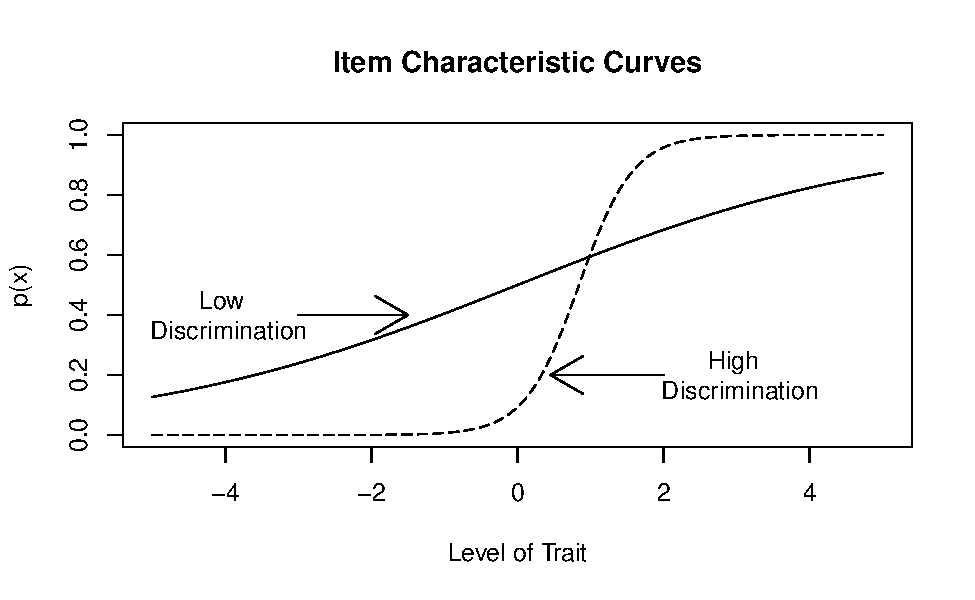
\includegraphics{ICC_project_files/figure-latex/unnamed-chunk-1-1.pdf}
\caption{\label{fig:unnamed-chunk-1}Item characteristic curve. X-axis indicates the trait level, and y-axis indicates the probability of getting the item correct.}
\end{figure}

Psychometricians who examine ICCs usually do it using Item Response Theory and Rasch models to get the parameters necessary to plot the curves. In a 2PL model, these would be item difficulty and item discrimination. Item difficulty is the necessary trait level for a respondent to have a 50/50 chance to answer the item correctly. Item discrimination is the degree to which an item can differentiate among individuals with low and high levels of the trait. From a Classical Test Theory (CTT) frame of thinking, the difficulty of an item is determined by looking at the p-values of the items, while discrimination is determined by checking the Cronbach alpha and the corrected item total correlations. Psychometricians who look at these CTT parameters don't typically use them to plot ICCs.There is no reason for them not to, since ICCs based on CTT parameters could provide information as valuable as those based on IRT or Rasch without the need of being familiar with these models and with how to compute the necessary estimates. Fan states in summary that IRT and CTT ``\ldots{} framework produce very similar item and person statistics'' (p.379).

There is research that shows that there is little difference between the parameters of both frameworks.@hambleton1993comparison concluded that ``no study provides enough empirical evidence on the extent of disparity between the two frameworks and the superiority of IRT over CTT despite the theoretical differences.''

Fan (1998) conducted a study to empirically test the differences between the two frameworks. According to him, ``The findings here simply show that the two measurement frameworks produced very similar item and person statistics both in terms of the comparability of item and person statistics between the two frameworks and in terms of the degree of invariance of item statistics from the two competing measurement frameworks.'' In his study, Fan (1998) looked at the correlations between ability estimates and item difficulty in CTT and all three IRT models. These correlations were very high, between high .80 and low .90. As of item discrimination, correlations were moderate to high, with only a few being very low.

He also looked at the item invariance for all models. In theory, the major advantage of IRT models over CTT is that the latter has a circular dependency between the item and person statistics, while IRT has no such dependency, which means that the item parameters don't depend on the sample and the person parameters don't depend on the set of items. This property of invariance is very important, since item estimates can be used regardless of the sample you are giving the test or assessment to. An item will always have the same level of difficulty regardless of who is responding, for example.

What Fan (1998) got on his study, however, shows empirical evidence against this supposed advantage of IRT against CTT. The CTT item difficulty and discrimination degrees of invariance were highly correlated with those of IRT, indicating that they were highly comparable.

Lord (2012) described a function that approximates the relationship between IRT parameters and the CTT discrimination index of an item-test biserial correlation:

\[a_i\cong \frac{r_i}{\sqrt{1-r_i^2}}\]

This formula wasn't intended for practical purposes but rather to assist in the conceptual comprehension of the discrimination parameter in IRT for people who were more familiar with CTT procedures. In an effort to move from the conceptual to a practical application, Kulas, Smith, and Xu (2017) proposed a modification that minimized the average residual (either \(a_i\) or \(r_i\), where \(r_i\) is the \emph{corrected} item-total \emph{point-biserial} correlation).

Simulations identified systematic slope and inflection differences across item with differing item difficulty values, so the formula was further changed to include the following modifiers This revised formula is used in the current presentation:

\[\hat{a_i}\cong[(.51 + .02z_g + .3z_g^2)r]+[(.57 - .009z_g + .19z_g^2)\frac{e^r-e^{-r}}{e-e^r}]\]

Where \(g\) is the absolute deviation from 50\% responding an item correctly and 50\% responding incorrectly (e.g., a ``p-value'' of .5). \(Z_g\) is the standard normal deviation associated with \(g\). The transformation of the standard p-value was recommended in order to scale this index along an interval-level metric more directly anaologous to the IRT \emph{b} parameter. Figure XX visualizes the re-specifications of Lord's formula at p-values (difficulty) of .5, .3 (or .7), and .1 (or .9).

\begin{figure}
\centering
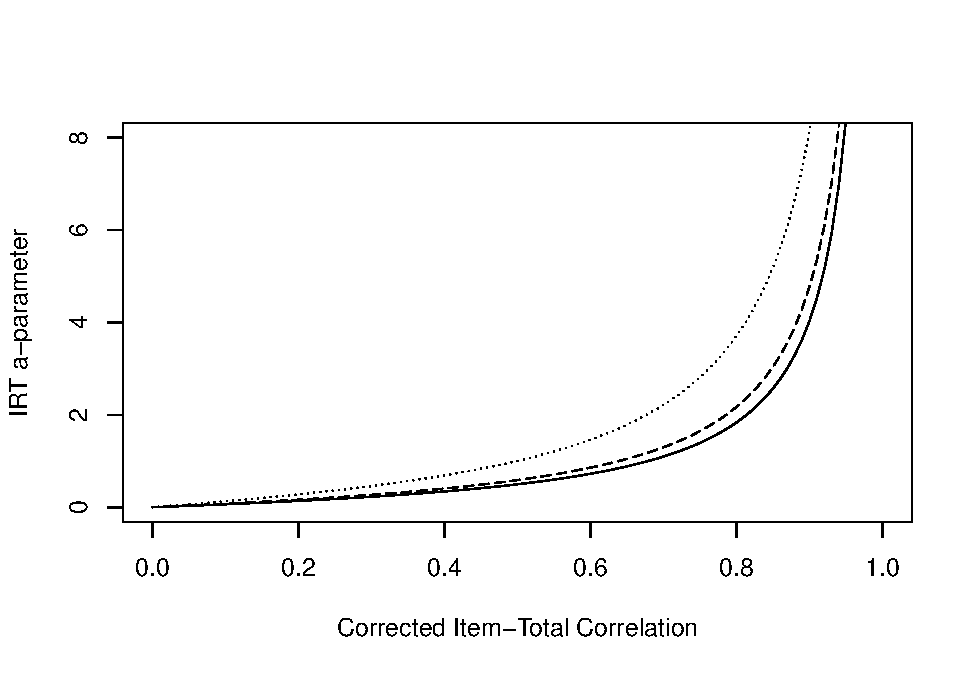
\includegraphics{ICC_project_files/figure-latex/acorrected-1.pdf}
\caption{\label{fig:acorrected}Functional relationship between the IRT \emph{a} parameter and the CTT corrected-item total correlation as a function of item difficulty (p-value; solid = .5, dashed = .3/.7, dotted = .1/.9).}
\end{figure}

As we can see, the higher the corrected item-total correlations, the higher the estimated IRT a-parameter (discrimination). Also, as the p-values (difficulty) deviates from 0, the relationship between the estimated IRT a-parameter and the corrected item-total correlations becomes stronger.

Practitioners and researchers that don't use IRT or Rasch models and instead opt to follow a CTT philosophy would benefit from having ICCs that use CTT statistics. This study intends to show evidence of the overlapping nature of CTT and IRT parameters when it comes to plotting ICCs.

\hypertarget{study-1---visual-of-discrimination-relationship}{%
\section{Study 1 - Visual of discrimination relationship}\label{study-1---visual-of-discrimination-relationship}}

The purpose of study 1 is to look at the visualizations resulting from Kulas, Smith, and Xu (2017) formula on simulated data. We hypothesize that the relationship between the estimated IRT a-parameter and the corrected item-total correlations will be stronger as the later deviates from 0, which would mean that the item has more discrimination.

\hypertarget{procedure-and-methods}{%
\subsection{Procedure and methods}\label{procedure-and-methods}}

We simulated data using Han (2007) software. Our sample was 10,000 observations, with a mean of 0 and a standard deviation of 1. The number of items were 100, with response categories of either correct or incorrect (1 and 0).The mean for the a parameter was 2, and the standard deviation 0.8. The mean for parameter b was 0 and the standard deviation 0.5.

\hypertarget{results}{%
\subsection{Results}\label{results}}

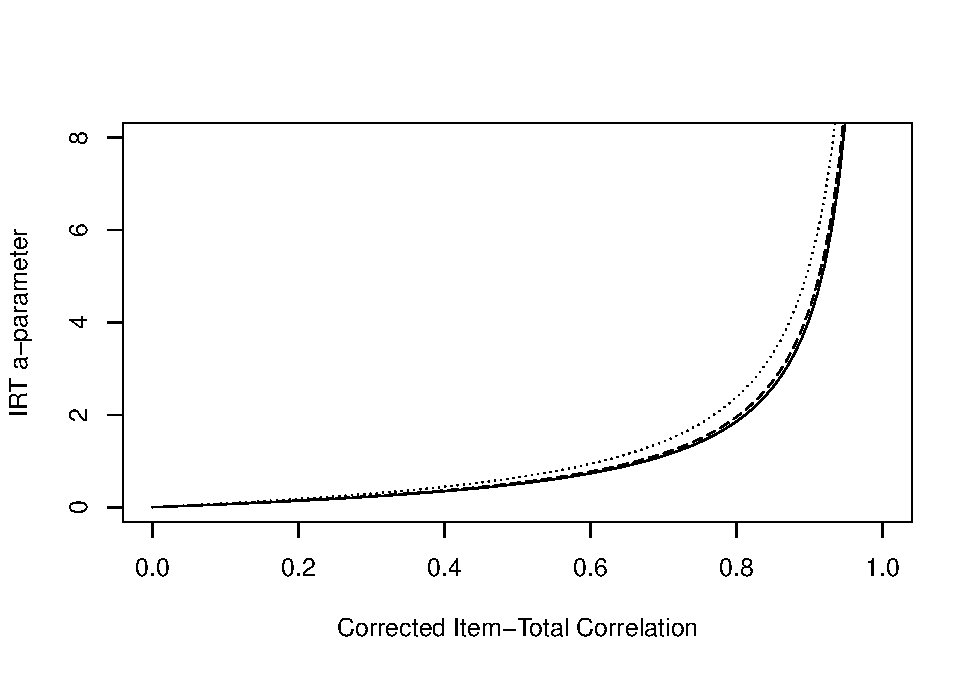
\includegraphics{ICC_project_files/figure-latex/acorrected simulation-1.pdf}
\newpage

\hypertarget{study-2---item-characteristic-curves-comparisons.}{%
\section{Study 2 - Item Characteristic Curves comparisons.}\label{study-2---item-characteristic-curves-comparisons.}}

The purpose of study 2 is to simulates a lot of test data and then generate ICCs based on the IRT model and then we compare that to our CTT estimates.

\hypertarget{procedure-and-materials}{%
\subsection{Procedure and materials}\label{procedure-and-materials}}

The same simulated data as in study 1 was used. The mirt package was used to compute the IRT statistics. The blue curves were plotted using 2PL IRT parameters (a and b), while the red curves were plotted using CTT parameters (p-values and corrected item-total correlations, modifying them with Kulas, Smith, and Xu (2017) formulas).

\hypertarget{results-1}{%
\subsection{Results}\label{results-1}}

We calculated the area between the curves plotted using CTT parameters and the curves with IRT parameters. The average difference for all 100 curves was 0.35.

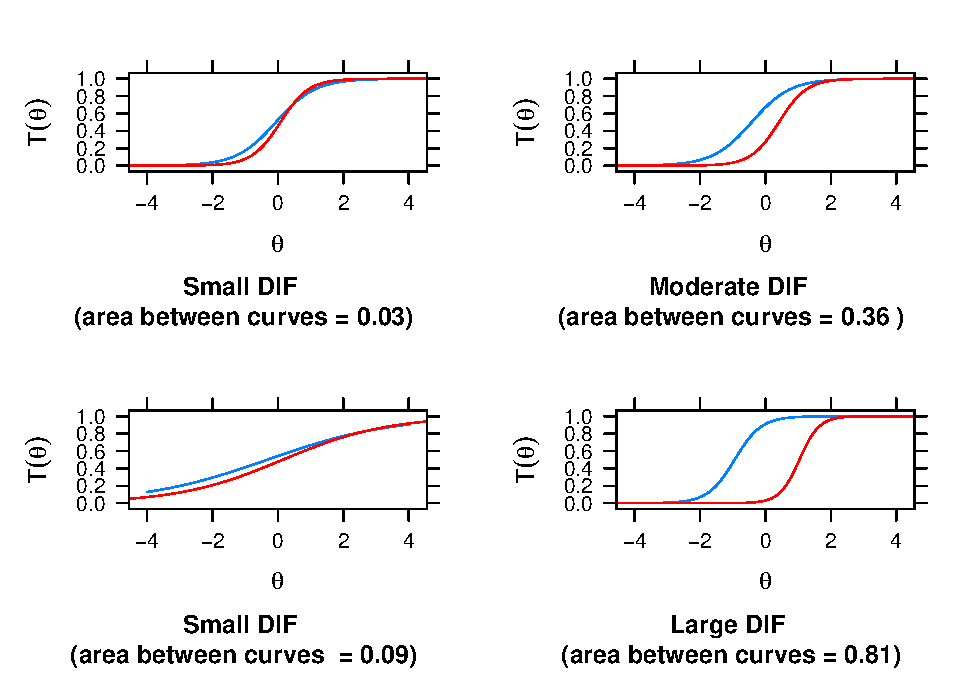
\includegraphics{ICC_project_files/figure-latex/plotting-1.pdf}

\begin{figure}
\centering
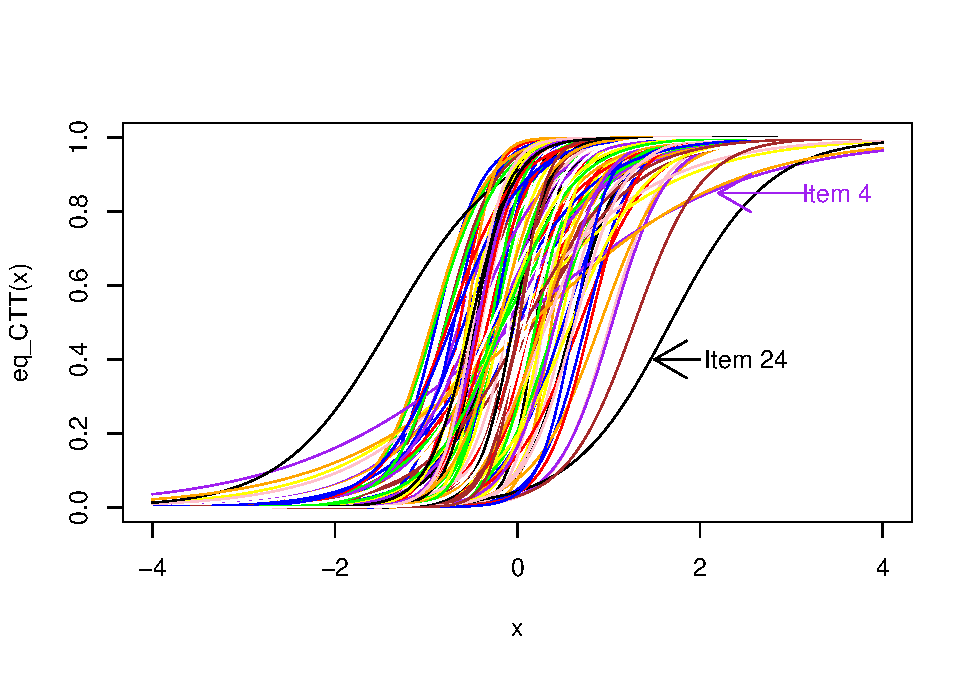
\includegraphics{ICC_project_files/figure-latex/AUC-1.pdf}
\caption{\label{fig:AUC}ICCs using CTT parameters}
\end{figure}

\begin{figure}
\centering
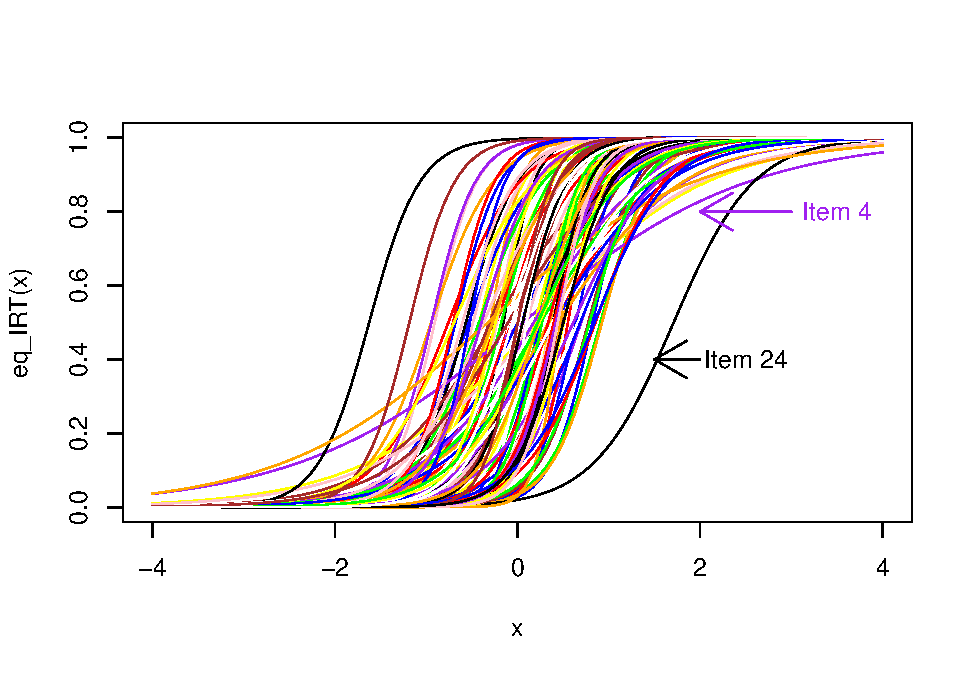
\includegraphics{ICC_project_files/figure-latex/irt curves-1.pdf}
\caption{(\#fig:irt curves)ICCs using IRT parameters}
\end{figure}

\hypertarget{results-2}{%
\section{Results}\label{results-2}}

\hypertarget{discussion}{%
\section{Discussion}\label{discussion}}

\newpage

\hypertarget{references}{%
\section{References}\label{references}}

\begingroup
\setlength{\parindent}{-0.5in}
\setlength{\leftskip}{0.5in}

\hypertarget{refs}{}
\begin{CSLReferences}{1}{0}
\leavevmode\hypertarget{ref-fan1998item}{}%
Fan, X. (1998). Item response theory and classical test theory: An empirical comparison of their item/person statistics. \emph{Educational and Psychological Measurement}, \emph{58}(3), 357--381.

\leavevmode\hypertarget{ref-han2007wingen3}{}%
Han, K. (2007). WinGen3: Windows software that generates IRT parameters and item responses {[}computer program{]}. \emph{Amherst, MA: Center for Educational Assessment, University of Massachusetts Amherst}.

\leavevmode\hypertarget{ref-kulas2017approximate}{}%
Kulas, J. T., Smith, J. A., \& Xu, H. (2017). Approximate functional relationship between IRT and CTT item discrimination indices: A simulation, validation, and practical extension of lord's (1980) formula. \emph{Journal of Applied Measurement}, \emph{18}(4), 393--407.

\leavevmode\hypertarget{ref-lord2012applications}{}%
Lord, F. M. (2012). \emph{Applications of item response theory to practical testing problems}. Routledge.

\end{CSLReferences}

\endgroup


\end{document}
